\documentclass{beamer}

\usepackage{graphicx}

\usetheme{Frankfurt}

\title{Slide shows in {\LaTeX} with Beamer}
\author{Javier Marquez}

\begin{document}

\maketitle

\section{Introduction}

\begin{frame}
	\frametitle{Roadmap}
	\begin{itemize}
		\item Frames \pause
		\item Beamer themes \pause
		\item Pauses and slides \pause
		\item Sections \pause
		\item Images \pause
		\item Columns
	\end{itemize}
\end{frame}

\section{Data}

\begin{frame}
	\frametitle{as dfasdf safd}

	adsfasdfadsfa
\end{frame}

\section{Aasdfa asdfasd}

\begin{frame}
	\frametitle{Another asdf frame}

	adsfasdffd
\end{frame}

\begin{frame}
	\frametitle{Images in Beamer}

	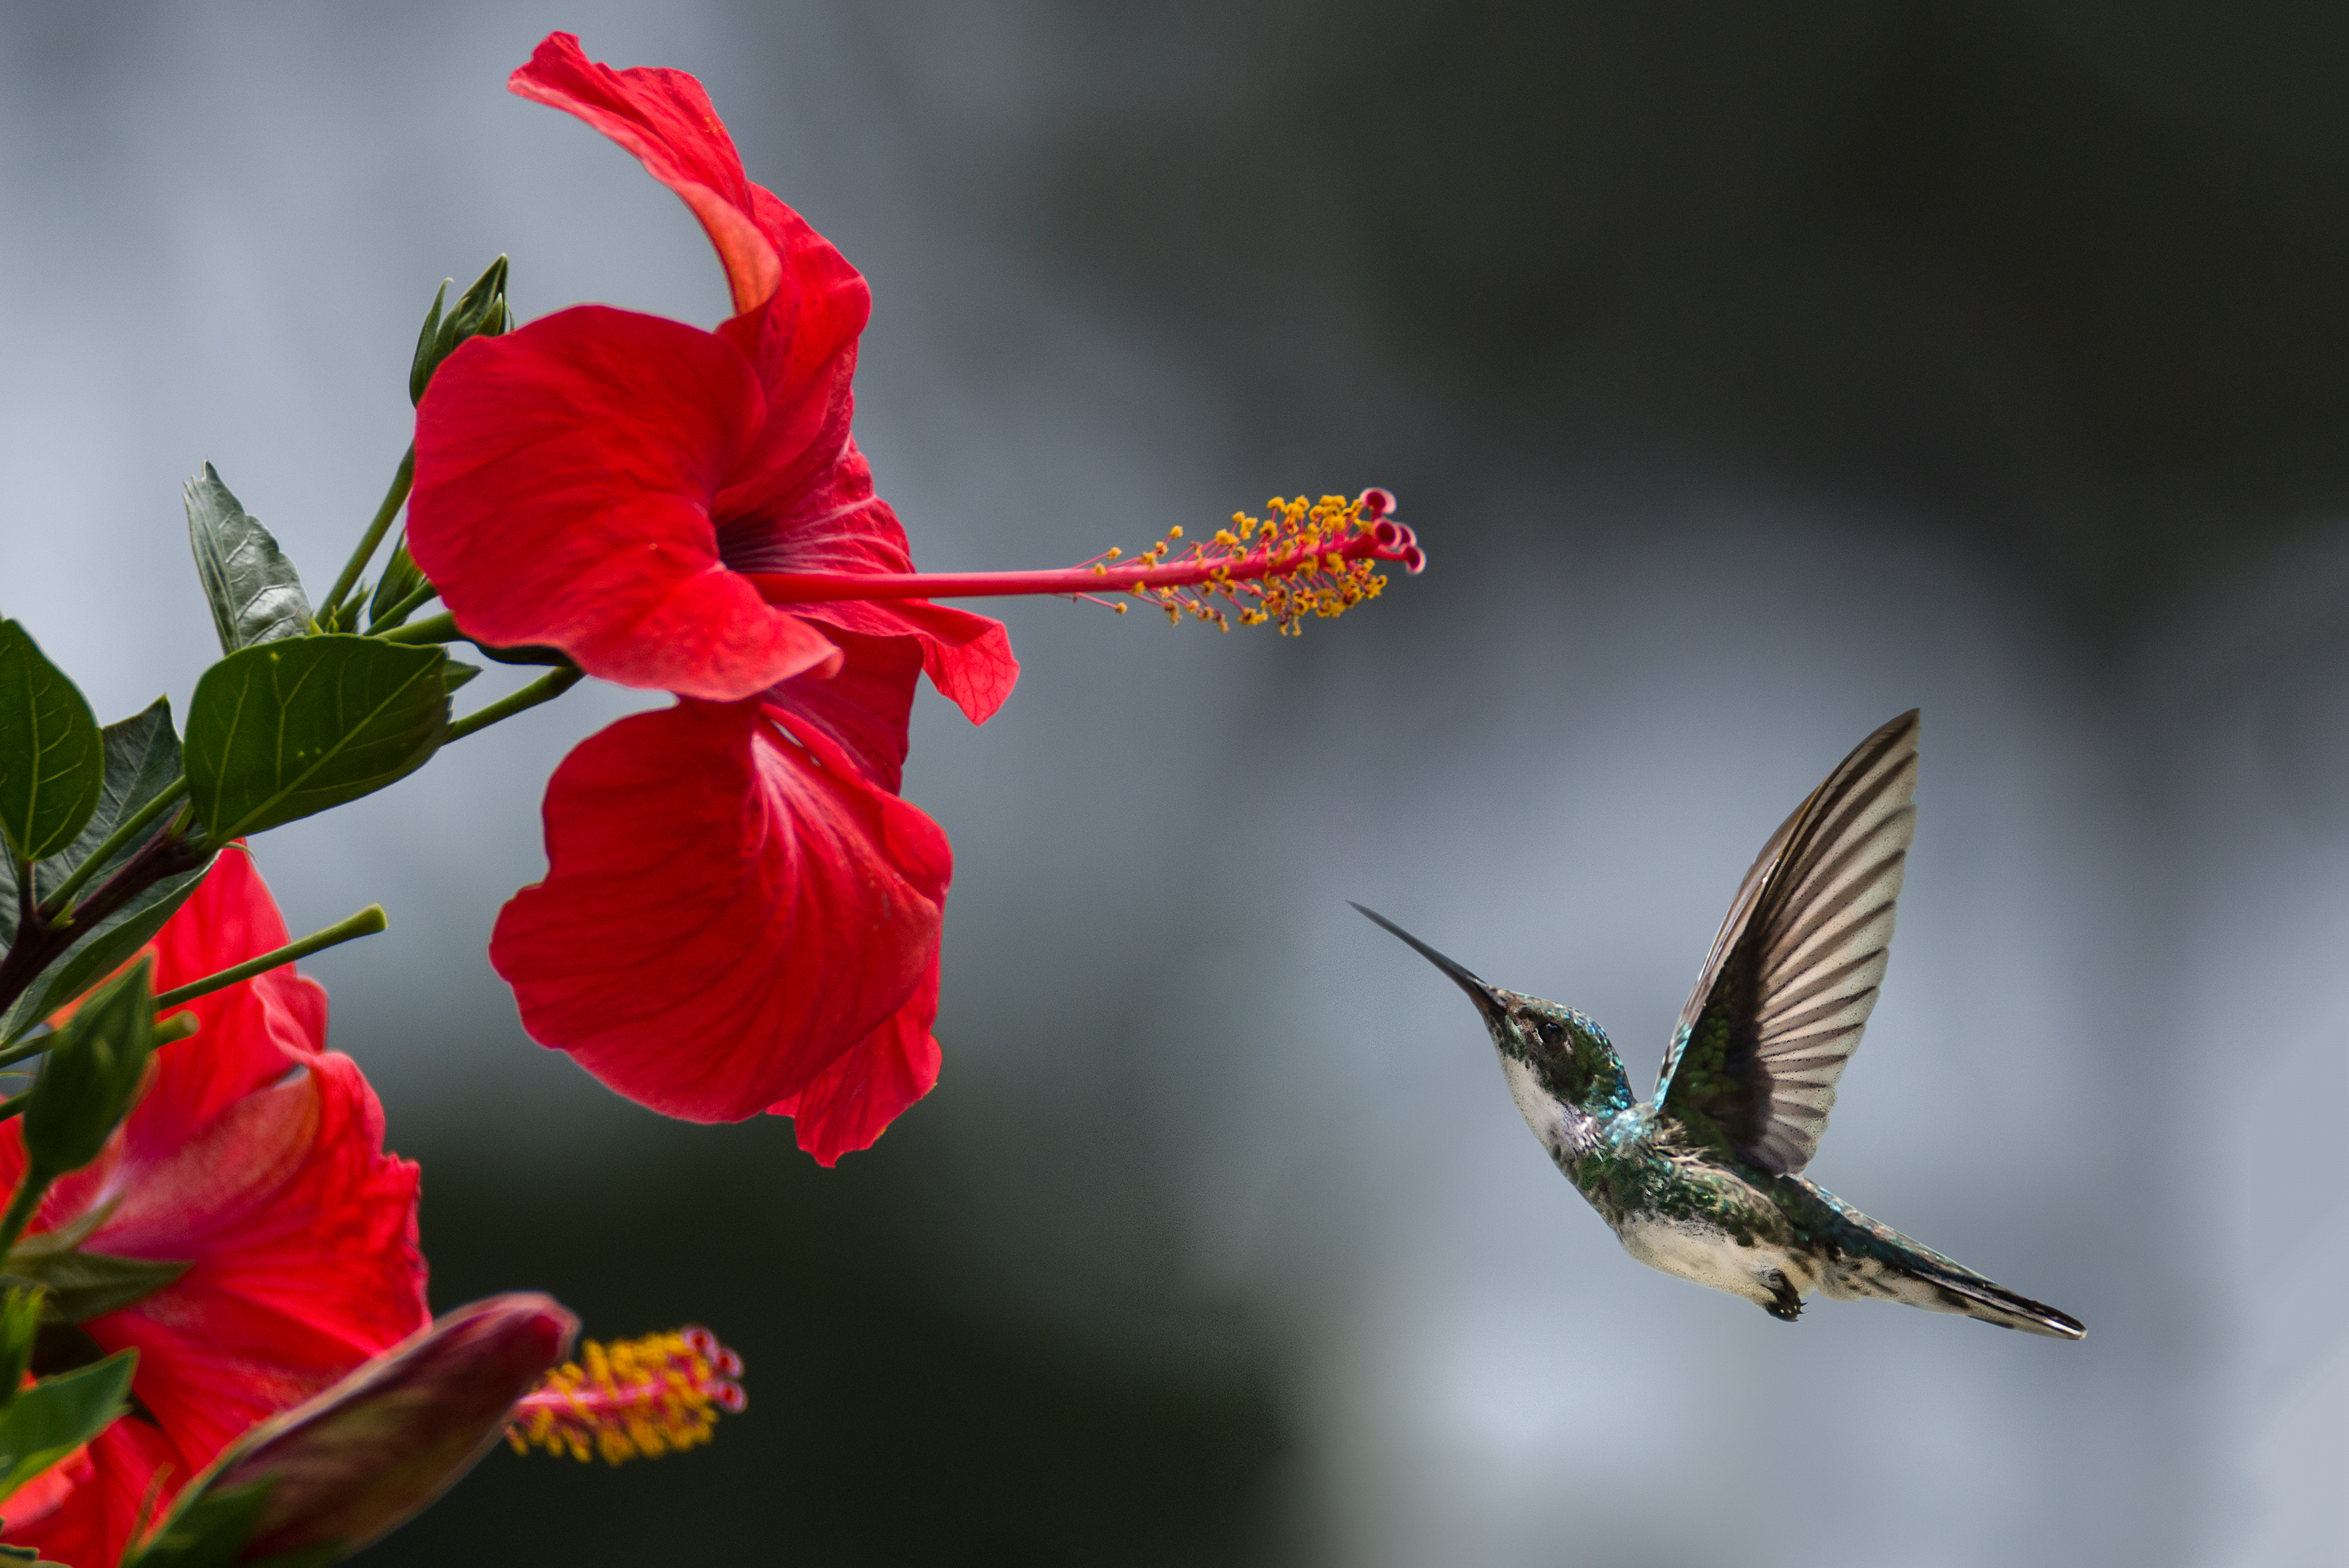
\includegraphics[width=.7\textwidth]{picture.jpeg}
\end{frame}

\begin{frame}
	\frametitle{Columns}

	\begin{columns}
		\column{.5\textwidth}

		asdf asdfas dfasdfk aslfaks asldfkasldkf

		\column{.5\textwidth}

		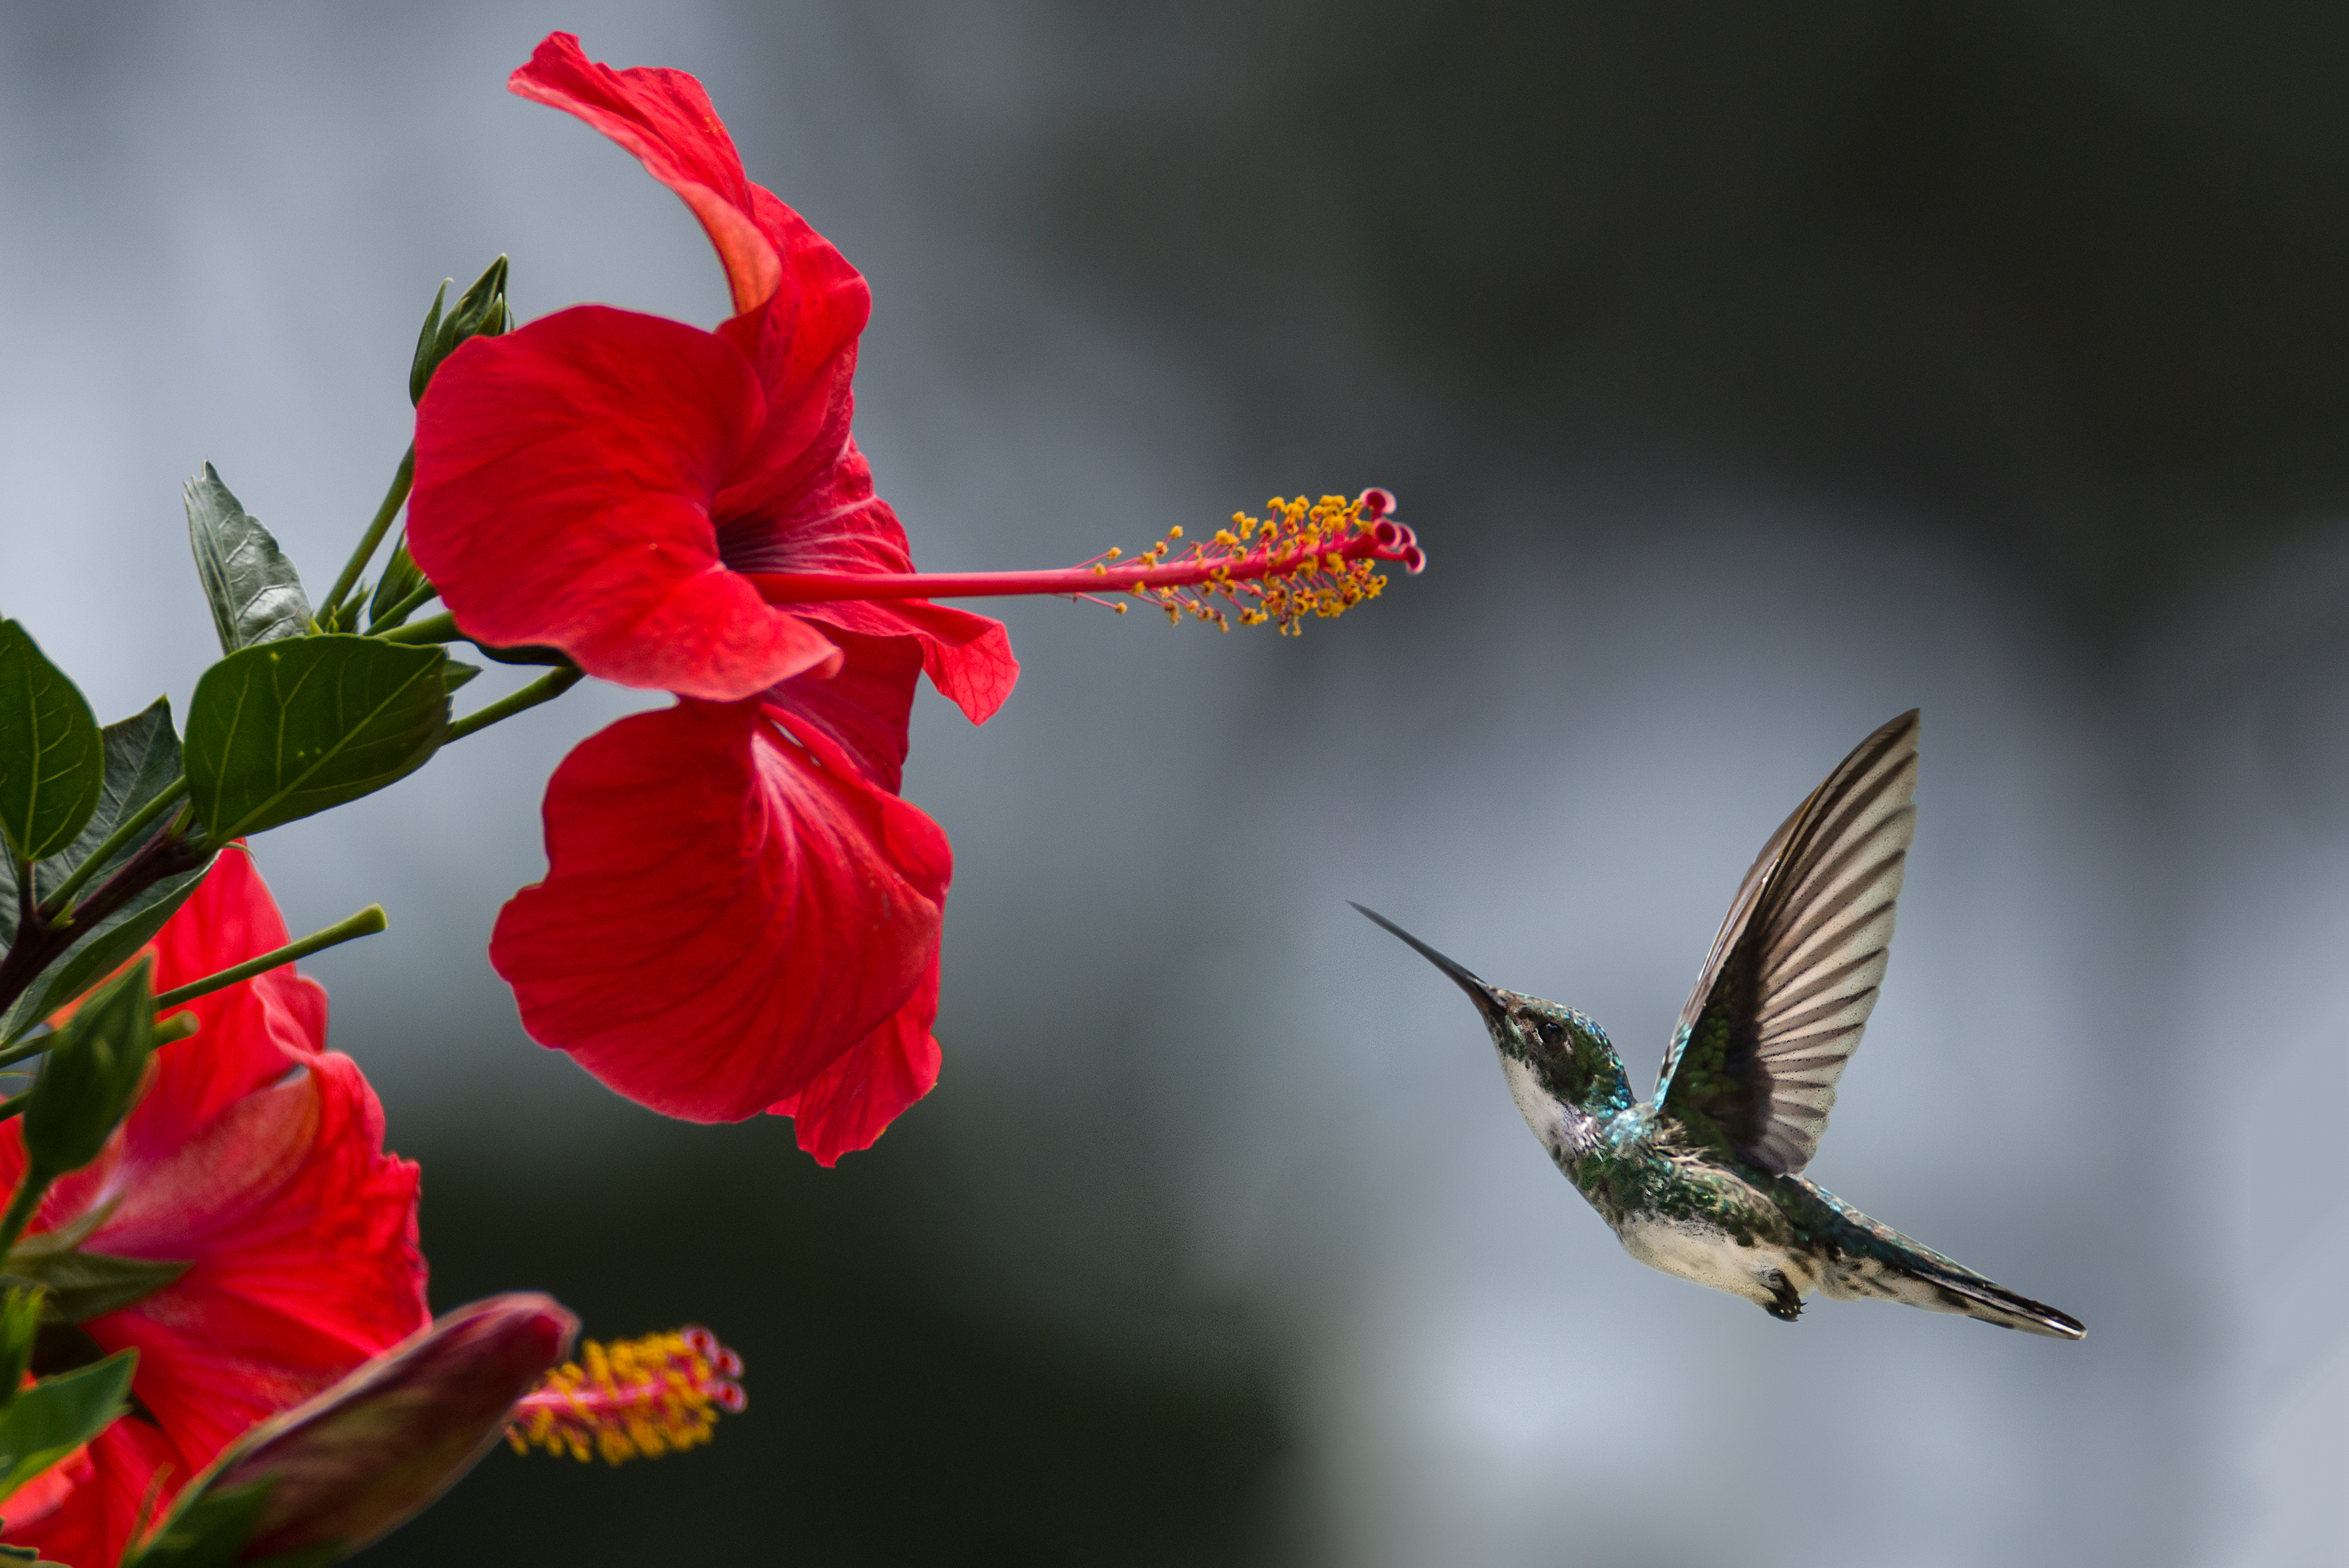
\includegraphics[width=\textwidth]{picture.jpeg}
	\end{columns}
\end{frame}

\end{document}
